\begin{figure}[H]
    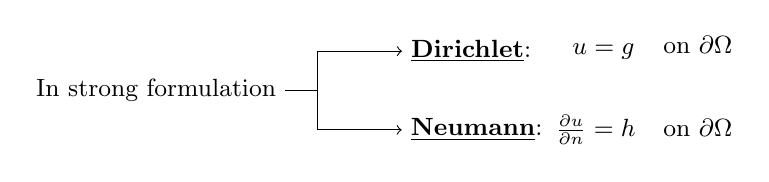
\begin{tikzpicture}

        \small

        \node at (0,0) (A) {In strong formulation};
        \node at (4,0.5) (B) {\underline{\textbf{Dirichlet}}:};
        \node at (4.07,-0.5) (C) {\underline{\textbf{Neumann}}:};

        \node at (5.68,0.5) () {$u=g$};
        \node at (5.58,-0.5) () {$\frac{\partial u}{\partial n}=h$};

        \node at (6.88,0.58) () {on $\partial\Omega$};
        \node at (6.88,-0.48) () {on $\partial\Omega$};

        \draw[->] (A) -- (2.05,0) -- (2.05,0.5) -- (B);
        \draw[->] (2.05,0) -- (2.05,-0.5) -- (C);

        \normalsize
    \end{tikzpicture}
\end{figure}